\chapter*{Biological overview}
\addcontentsline{toc}{chapter}{Biological overview}
The butterfly effect is somewhat present in our body too. A tiny malfunction in one area can lead to
serious diseases. Neurological diseases like Schizophrenia, Autism, Fraser syndrome and many more
rely on the wiring and connections of the brain. Moreover the mentioned diseases have been linked to
excitatory synapses. The postsynaptic density (PSD) of a synapse is a dense and active network of
proteins. Proteins in this network regulate, guide and anchor the receptors to the membrane. A large
number of PSD proteins contain the domain called PDZ. As a reminder: a domain is a building block of
a protein that carries an independent function and is usually encoded by a separate (set of) exon(s). The
PDZ domain is specialised for binding, creating the nodes of the network. Proteins containing PDZ
domains  influence the  function  of the PSD, synapses  and can  have a  clear  impact in multiple
neurological diseases
\begin{figure}
\centering
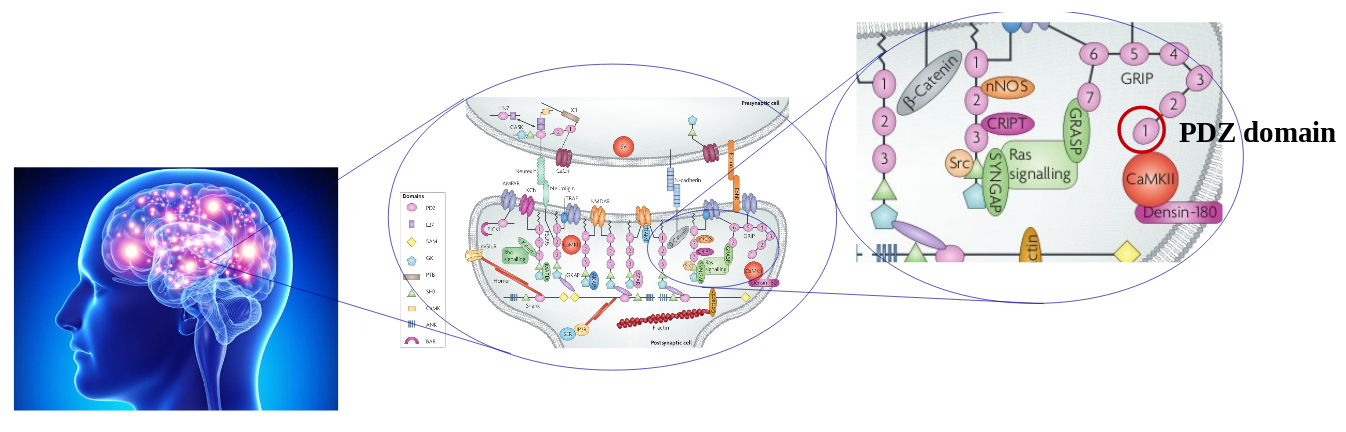
\includegraphics[width=\textwidth]{PDZ.png}
\caption{\emph{Proteins containing PDZ
domains  influence the  function  of the PSD, synapses  and can  have a  clear  impact in multiple
neurological diseases.}
Image source \href{https://wiki.itk.ppke.hu/twiki/pub/PPKE/BevBioInfo2016/bioinfo_p2016.pdf}{Assignment description}
%
}
\end{figure}